% Dépendences : 
% pip install pygments
% Python3

% Installation de pip : (Windows)
% wget https://bootstrap.pypa.io/get-pip.py
% python3 get-pip.py
% Rajout dans le PATH, cf. message

% Compilation : 
% 1 - pdflatex --shell-escape rapport.tex
% 2 - bibtex --shell-escape rapport.aux
% 3 - pdflatex --shell-escape rapport.tex


% Citations de sources bibliographiques
% http://merkel.texture.rocks/Latex/natbib.php?lang=fr

% Documentation classe 
% https://www.elsevier.com/__data/assets/pdf_file/0009/56844/elsdoc2.pdf
\documentclass[3p, twocolumn]{elsarticle}
\usepackage[T1]{fontenc}
\usepackage[utf8]{inputenc}
\usepackage{csquotes}
\usepackage[french]{babel}
\usepackage{fancyhdr}
\usepackage{physics}
\usepackage{titlesec} % titlespacing %
\usepackage{listings} % lstnewenvironment %
\usepackage{textcomp}
\usepackage{regexpatch}
\usepackage[usenames,dvipsnames,svgnames,table]{xcolor}
\usepackage{parskip}
\usepackage{graphicx}
\usepackage{pdfpages}
\usepackage{caption}
\usepackage{titletoc}
\usepackage{mathrsfs}
\usepackage[table]{xcolor}
\usepackage{minted}
\usepackage[french]{algorithm2e}% http://tug.ctan.org/macros/latex/contrib/algorithm2e/doc/algorithm2e.pdf
\usepackage{amsmath,amssymb,amsfonts}
\usepackage{graphicx}
\usepackage{textcomp}
\usepackage{xcolor}
\usepackage[hidelinks]{hyperref}
\usepackage[toc,page]{appendix}
\renewcommand{\appendixtocname}{Annexes}
\renewcommand{\appendixpagename}{Annexes}
\DeclareMathOperator{\Hessian}{H}
\DeclareMathOperator{\Jacobian}{J}
\hypersetup{
  colorlinks = false,
  citecolor=black,
  filecolor=black,
  linkcolor=black,
  urlcolor=black
}
\newtheorem{thm}{Théorème}
\newtheorem{lem}[thm]{Lemme}
\newtheorem{definition}{Définition}[section]
\newdefinition{rmk}{Remarque}[section]
\newdefinition{exemple}{Exemple}[section]
\newproof{pf}{Preuve}[section]

\newcounter{linecounter}
\newcommand{\linenumbering}{\ifthenelse{\value{linecounter}<10}{(0\arabic{linecounter})}{(\arabic{linecounter})}}
\renewcommand{\line}[1]{\refstepcounter{linecounter}\label{#1}\linenumbering}
\newcommand{\resetline}[1]{\setcounter{linecounter}{0}#1}
\renewcommand{\thelinecounter}{\ifnum \value{linecounter} > 9\else 0\fi \arabic{linecounter}}

% Enlever le footer spécifique à Elsevier

\keywordtitle{Mots-clés\,}
\abstracttitle{Résumé}

\makeatletter
\regexpatchcmd*{\@makecaption}{:}{\cA:}{}{}
\regexpatchcmd*{\keyword}{:}{\cA:}{}{}
\def\ps@pprintTitle{%
 \let\@oddhead\@empty
 \let\@evenhead\@empty
 \def\@oddfoot{}%
 \let\@evenfoot\@oddfoot}
% fix english
\xpatchcmd{\printFirstPageNotes}
  {Email addresses}
  {Adresses email}{}{}
\xpatchcmd{\printFirstPageNotes}
  {Email address}
  {Adresse email}{}{}
\regexpatchcmd*{\printFirstPageNotes}{:}{\cA -}{}{}
\makeatother

\begin{document}
\nocite{arxiv:kovalev2019stochastic}
\begin{frontmatter}
    \title{Méthode de Newton et de Quasi-Newton BFGS (Algorithme de BRoyden, Fletcher, Goldfarb et Shanno)}
    \author{Mathilde Rineau}
    \author{Mathilde Le Moel}
    \author{Pascal Quach}
    \author{Félix Poullet-Pagès}

    \begin{abstract}
        La méthode de Newton est une méthode itérative de recherche d'un zéro d'une fonction $g$, qui se repose sur la méthode du point fixe. Elle requiert cependant le calcul coûteux de la dérivée ou matrice jacobienne de $g$ dans le cas d'une fonction à plusieurs variables, et également son inversion. Les méthodes sont qualifiées de quasi-Newton lorsque la matrice jacobienne - généralement son inverse - sont remplacées par une approximation. Appliquée à un problème d'optimisation mono-objectif libre, où l'on cherche l'optimum d'une fonction $f:\mathbb{R}^n\rightarrow \mathbb{R}$, la méthode de Newton force le calcul de la matrice hessienne de $f$, car on cherche les zéros du gradient de $f$. La méthode de Broyden-Fletcher-Goldfarb-Shanno (BFGS) est une méthode quasi-Newton qui se repose sur l'approximation de la matrice hessienne - ou son inverse - par analyse des gradients successifs. La matrice hessienne n'est pas calculée à chaque itération de la méthode, mais mise à jour itérativement en prenant une estimation de la matrice hessienne initiale.
    \end{abstract}
\end{frontmatter}

\tableofcontents

\section{Notations}
\begin{enumerate}
    \item $\Jacobian_{f}(x)$ désigne la matrice jacobienne de la fonction $f$ évaluée en $x$.
    \item $\nabla f(x)$ désigne le gradient de la fonction $f$ évaluée en $x$.
    \item $\Hessian_{f}(x)$ désigne la matrice hessienne de la fonction $f$ évaluée en $x$.
    \item $\nabla^2_{f}(x)$ désigne la dérivée du gradient de la fonction $f$ évaluée en $x$.
\end{enumerate}

\section{Méthode de Newton}
\subsection{Origines}
La méthode de Newton apparaît pour la première fois au XVIIème siècle dans l'ouvrage \emph{De analysi per aequationes numero terminorum infinitas} (1669), puis une seconde fois dans \textit{La méthode des fluxions\footnote{Les fluxions représentent des dérivées}, et les suites infinies}\footnote{Voir \cite{book:newtonfluxions}}, tous deux écrits par Isaac Newton. Elle est à l'époque appliquée au cas particulier des recherches des racines d'un polynôme. Ses travaux ne seront malheureusement publiés que de façon posthume à partir de 1736. Cette méthode est simplifiée par Joseph Raphson dans \textit{Analysis aequationum universalis} (1690), et c'est généralement la version de Raphson qui est utilisée aujourd'hui. Pour ces raisons, on a tendance à parler de la méthode de Newton-Raphson. Les travaux de Thomas Simpson élargissent cette méthode itérative à la recherche de racines d'un plus grande nombre d'équations, notamment les équations non linéaires.
\begin{figure}[htbp]
    \centering
    \includegraphics[width = 0.3\textwidth]{La_méthode_des_fluxions_et_[...]Newton_Isaac_bpt6k62411f_40.jpg}
    \caption{Extrait de l'ouvrage \textit{La méthode
            des fluxions, et les suites infinies} expliquant la méthode de Newton}
    \label{fig:fluxion_newton_method}
\end{figure}

\subsection{Principe}
La méthode de Newton-Raphson est une méthode de recherche des racines d'une fonction à valeurs réelles.
\begin{thm}
    \'Etant donné une fonction $G: \Omega\subset\mathbb{R}^n\longrightarrow \mathbb{R}$, $G$ différentiable et une valeur initiale $x_0\in \Omega$ donnée, alors la suite $(x_k)_{k\in \mathbb{N}}$ définie par
    \begin{equation}
        x_{k+1} = x_k - \Jacobian^{-1}_G(x_k)\cdot G(x_k)
        \label{eq:iteration-newton-rn}
    \end{equation}
    converge vers une racine $x_*$ de $G$, à condition que $x_0$ soit suffisamment proche de $x_*$.
\end{thm}
\begin{rmk}
    $\Jacobian_G$ est préférablement inversible. Si la matrice n'est pas carrée, on peut se servir du pseudo-inverse de matrices non-carrés; à gauche s'il y a plus de contraintes que de variables; à droite s'il y a plus de variables que de contraintes. Si la matrice est carrée non inversible, on peut se servir du pseudo-inverse de Moore-Penrose.
    \begin{exemple}
        Trouver les racines de $F
            \begin{pmatrix}
                x \\y
            \end{pmatrix}
            =
            \begin{pmatrix}
                x^2+y^2-1 \\
                y+x
            \end{pmatrix}$ est un problème "bien contraint", la matrice jacobienne est inversible. Si l'on décide de rajouter une contrainte, par exemple $y-\frac{\sqrt2}{2}$, alors le jacobien n'est pas carré, on peut se servir du pseudo-inverse pour appliquer la méthode de Newton-Raphson.
    \end{exemple}
\end{rmk}
\begin{rmk}
    Il est important que la fonction $G$ admette un développement de Taylor d'ordre 1 dans un voisinage des racines $x_*$. En effet, l'existence de ce développement justifie en partie la convergence de la méthode itérative. Itérativement, on souhaite contraindre la suite $(x_k)_{k\in \mathbb{N}}$ telle qu'à toute itération $k$, $G(x_{k+1})=0$. On considère le développement de Taylor \textit{d'ordre 1} au voisinage de $x_{k}$.
    \begin{equation*}
        G(x_{k+1})\simeq G(x_k)+\Jacobian_G(x_k)\cdot(x_{k+1}-x_k)
    \end{equation*}
    Dans l'idée, pour s'approcher d'une racine de $G$, on applique la contrainte souhaitée $G(x_{k+1})=0$, et on en déduit l'expression de l'équation \ref{eq:iteration-newton-rn}. L'erreur à chaque itération est dûe à l'approximation par le développement de Taylor : on a négligé son reste.
\end{rmk}
\begin{rmk}
    La méthode de Newton-Raphson peut être appliquée aux fonctions holomorphes, fonctions à valeurs complexes, définies et dérivables en tout point d'un ouvert de $\mathbb{C}$.
\end{rmk}
\begin{rmk}
    Il existe des variations sans paramétrisation nécessaire de la méthode de Newton-Raphson pour l'optimisation libre multi-objective. \cite{art:Fliege_Drummond_Svaiter_2009}
\end{rmk}
\subsection{Interprétation géométrique}
Pour mieux comprendre cette méthode itérative, il est plus simple de raisonner en deux dimensions. On considère la fonction $g :\Omega\subset\mathbb R^2 \rightarrow \mathbb R$.

La formule itérative équivalente est la suivante :
\begin{equation}
    x_{k+1}=x_k-\frac{g(x_k)}{g'(x_k)}
    \label{eq:iteration-newton-r2}
\end{equation}
En passant tous les membres à gauche dans l'équation \ref{eq:iteration-newton-r2}, on obtient $g'(x_k)(x_{k+1}-x_k)+g(x_k)=0$. On reconnaît ici l'équation de la tangente à $g$ en $x=x_k$ évaluée au point $(x_{k+1},0)$.
Ce point correspond à l'intersection entre la tangente à $g$ en $x_k$ et la droite des abscisses.

La figure \ref{fig:nr-iterations-1} fournit un exemple visuel des itérations de la méthode de Newton-Raphson en deux dimensions. La fonction $g$ est définie par $g(x)=\frac{1}{12}x^3+\frac18x^2-3x$, et on choisit comme valeur de recherche initiale $x_0=-3.5$. On dessine les tangentes successives, et leurs intersections, jusqu'à s'approcher raisonnablement d'une racine de $g$.

\begin{figure}[htbp]
    \centering
    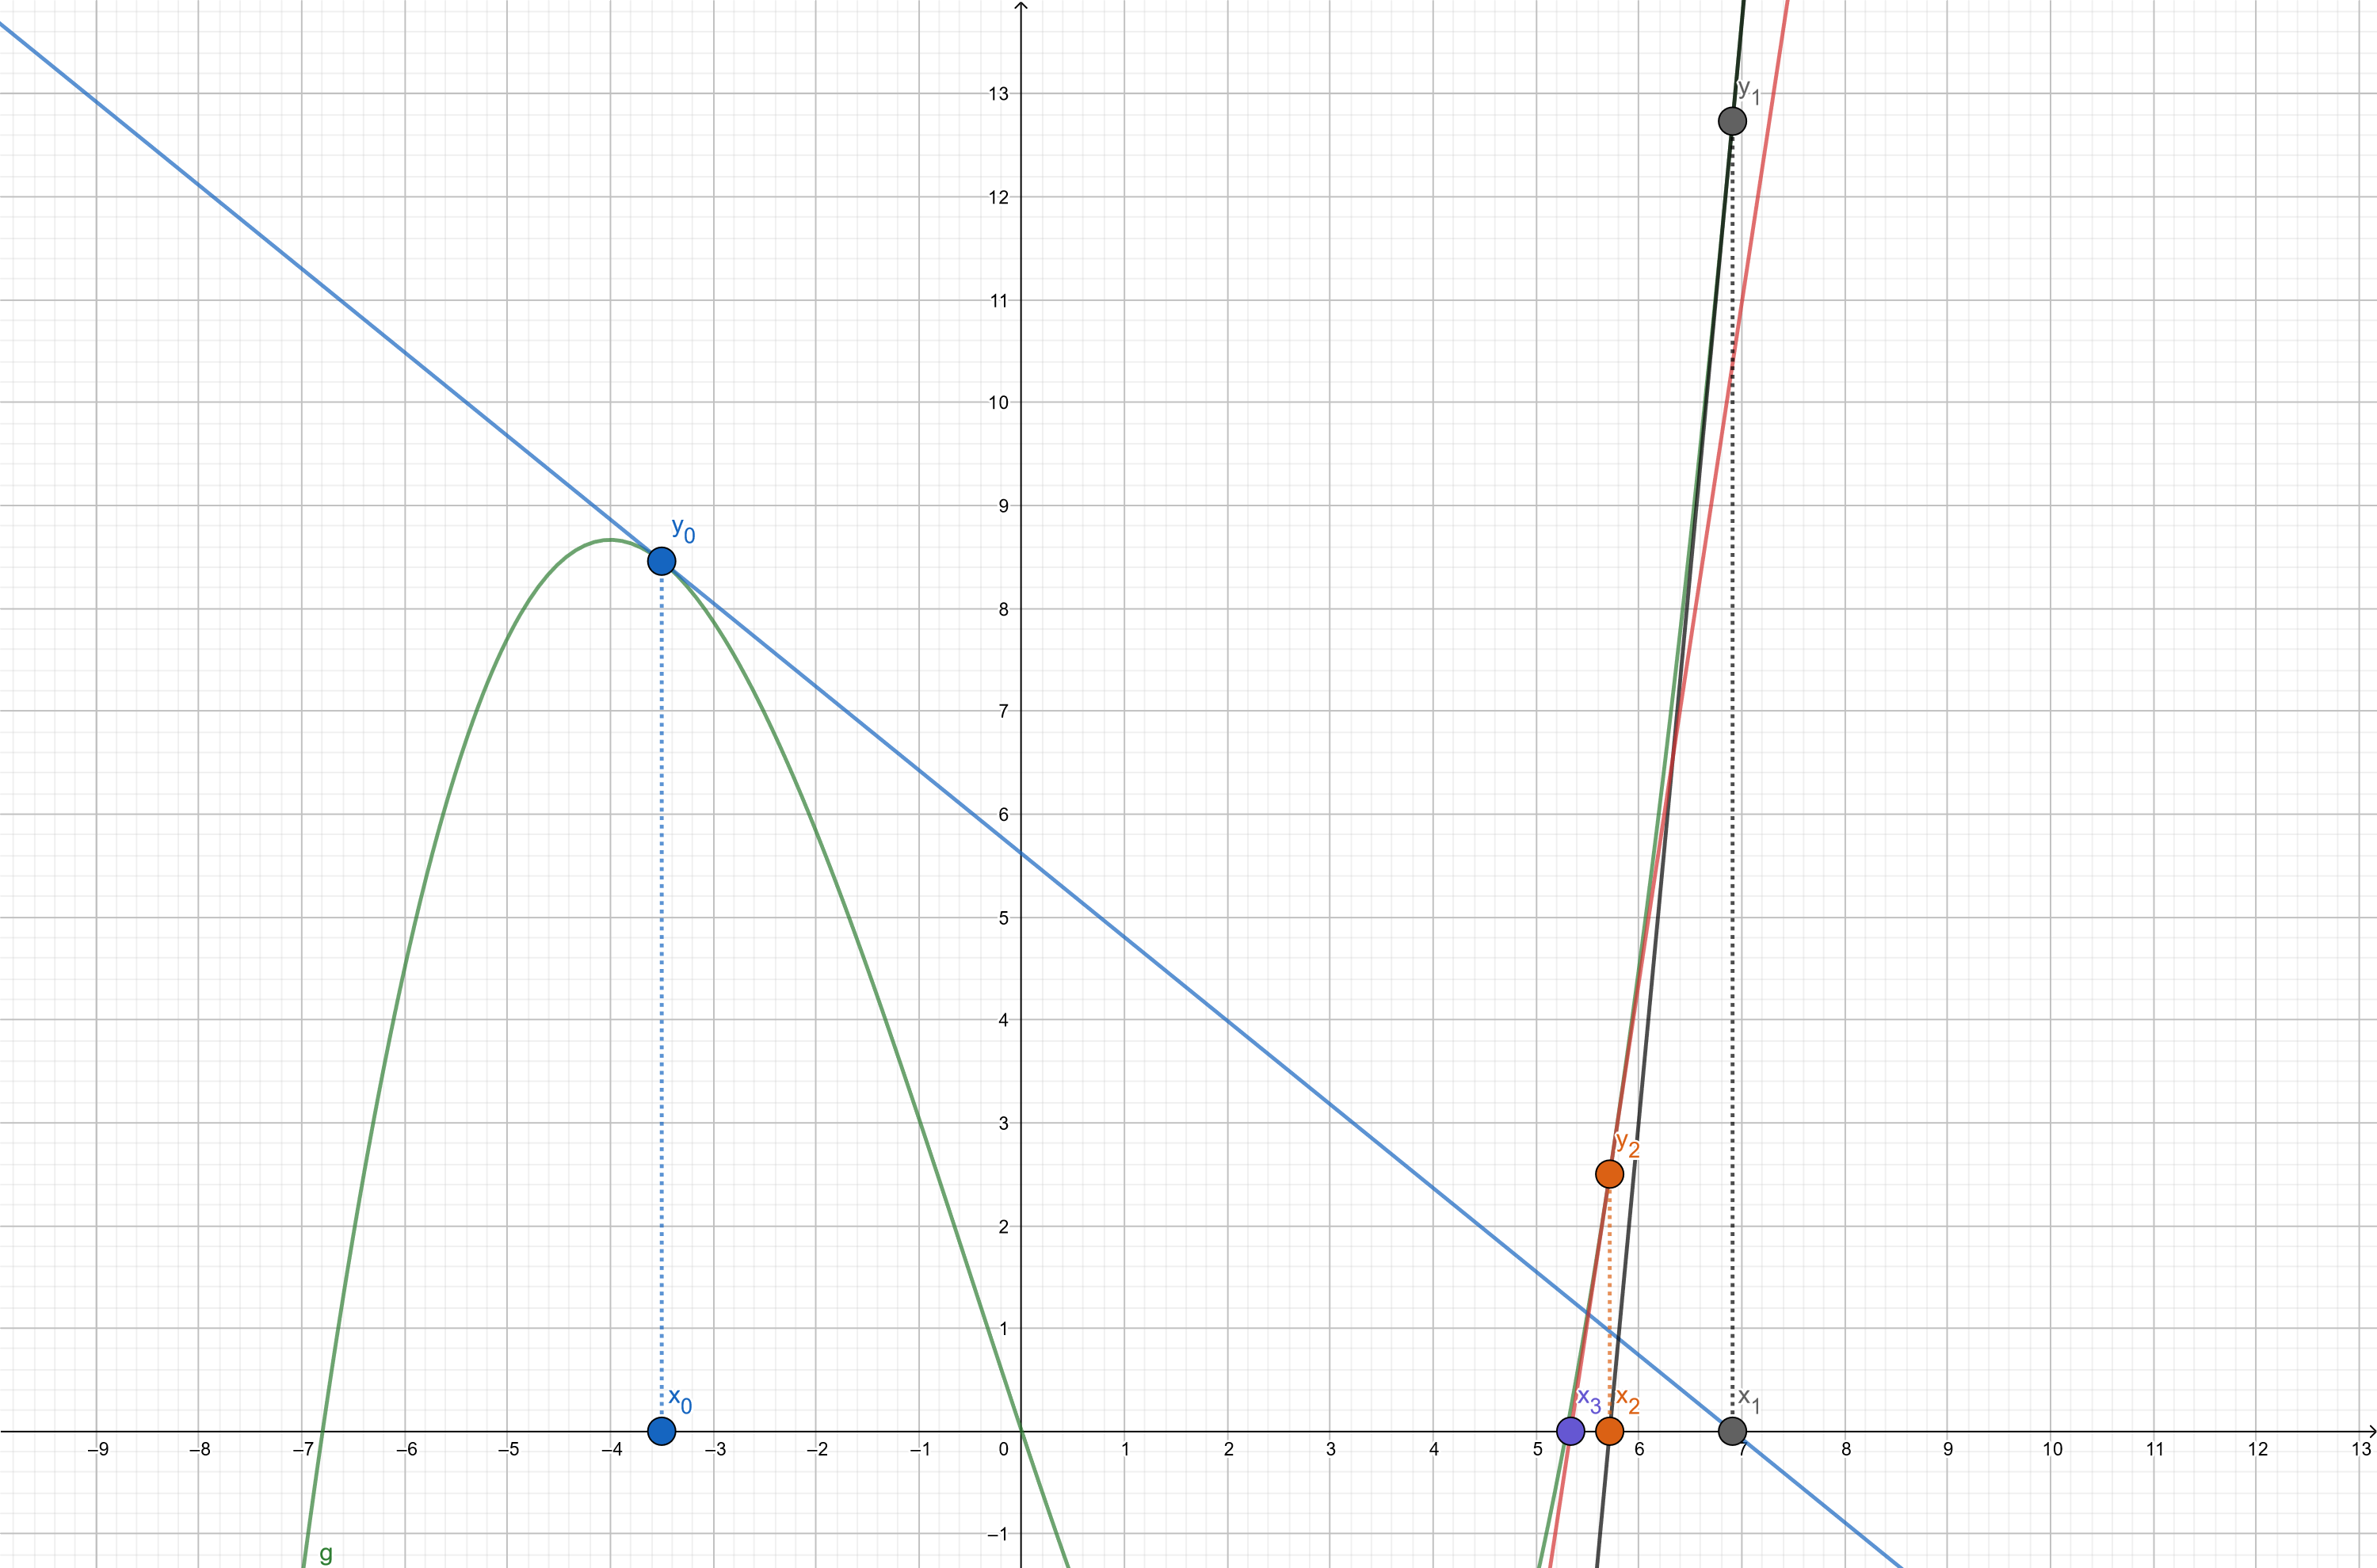
\includegraphics[width = 0.3\textwidth]{iteration-newton-1.png}
    \caption{Itérations de l'algorithme de Newton-Raphson pour la fonction $g$ définie par $g(x)=\frac{1}{12}x^3+\frac18x^2-3x$ telle que $x_0=-3.5$}
    \label{fig:nr-iterations-1}
\end{figure}

\begin{rmk}
    Le choix de la valeur de recherche initiale est important. Si l'on choisit $x_0=-4$, la pente de la tangente de $g$ en $x_0$ est nulle, et les itérations suivantes ne sont pas définies car la dérivée est nulle : la méthode itérative s'arrête. Ce choix a tout autant d'importance en dimensions supérieures à 2.
\end{rmk}


\subsection{Qualités et faiblesses}
\subsubsection{Vitesse de convergence}
La convergence est d'ordre quadratique au voisinage d'une solution. Si la suite converge, alors :

\begin{equation*}
    \lVert x_{k+1}-x^{*}\rVert \leq \gamma\lVert x_{k}- x^{*}\rVert^{2}, \gamma >0
    \label{eq:convergence-nr}
\end{equation*}

La méthode de Newton-Raphson converge quadratiquement au voisinage d'une solution, ce qui est remarquable. Malheureusement, cet ordre de convergence n'est valable que localement, ce qui limite son intérêt. De plus, il est généralement difficile d'expliciter "le voisinage de $x_*$".

\subsubsection{Cas de non convergence}
Dans certains cas, la méthode de Newton-Raphson ne converge pas.

\textbf{Domaine de définition} - Le calcul de $x_{k+1}$ peut mener à une valeur en dehors du domaine de définition $\Omega$ de $G$.

\textbf{Différentiabilité} - Si le gradient de la fonction $G$, $\Jacobian_G(x)$ a un comportement anormal, e.g. il n'est pas définie au voisinage d'une racine $x_*$, c'est-à-dire que $G$ n'est pas différentiable en $x_*$, alors la méthode ne peut pas converger.

\textbf{Optima locaux} - Au cours des itérations de la méthode, l'algorithme peut éventuellement s'arrêter sur un optimum. La méthode oscille (ou s'arrête si on doit diviser par 0), car la matrice jacobienne sera nul. La matrice jacobienne peut être nulle, dans ce cas-là la méthode est "bloquée" : $x_{k+1} = x_k$. Ce cas de non-convergence correspond en deux dimensions à la pente nulle de la tangente en $x_k$.

\textbf{Valeur initiale} - Toutefois, la non-convergence de la méthode de Newton-Raphson est le plus souvent due au mauvais choix de la valeur initiale $x_{0}$. Il est important d'itérer à partir d'une estimation raisonnable de la solution voulue.

\textbf{Convergence} - En somme, pour une fonction quelconque, il n'existe aucune garantie que la méthode de Newton-Raphson converge. Il faudra s'assurer que la fonction ait certaines propriétés particulières - notamment sa stricte convexité - pour appliquer la méthode de Newton-Raphson à un problème d'optimisation.

\begin{exemple}
    On considère la fonction $G:\mathbb R^n\rightarrow \mathbb R^n$ définie par $G(x)=\left(\lvert x_i\rvert^{\frac12}\right)_{1\leq i\leq n}$. La méthode itérative de Newton-Raphson mène à $x_{k+1}=-x_k$. \footnote{Les détails du calcul sont précisés dans l'annexe \ref{ap:calcul-exemple-nr}.}
    \label{ex:newton-raphson-non-differentiable}
    La méthode Newton-Raphson ne converge pas, et on oscille entre deux points. Effectivement, comme $G$ n'est pas différentiable en $x_k=\overrightarrow 0$, la matrice jacobienne n'y est pas définie. Pour toute valeur $x_0\neq \overrightarrow 0$, l'algorithme ne convergera pas. En figure \ref{fig:nr-iterations-2}, les itérations pour la fonction $G$ lorsque $n=1$.
    \begin{figure}[htbp]
        \centering
        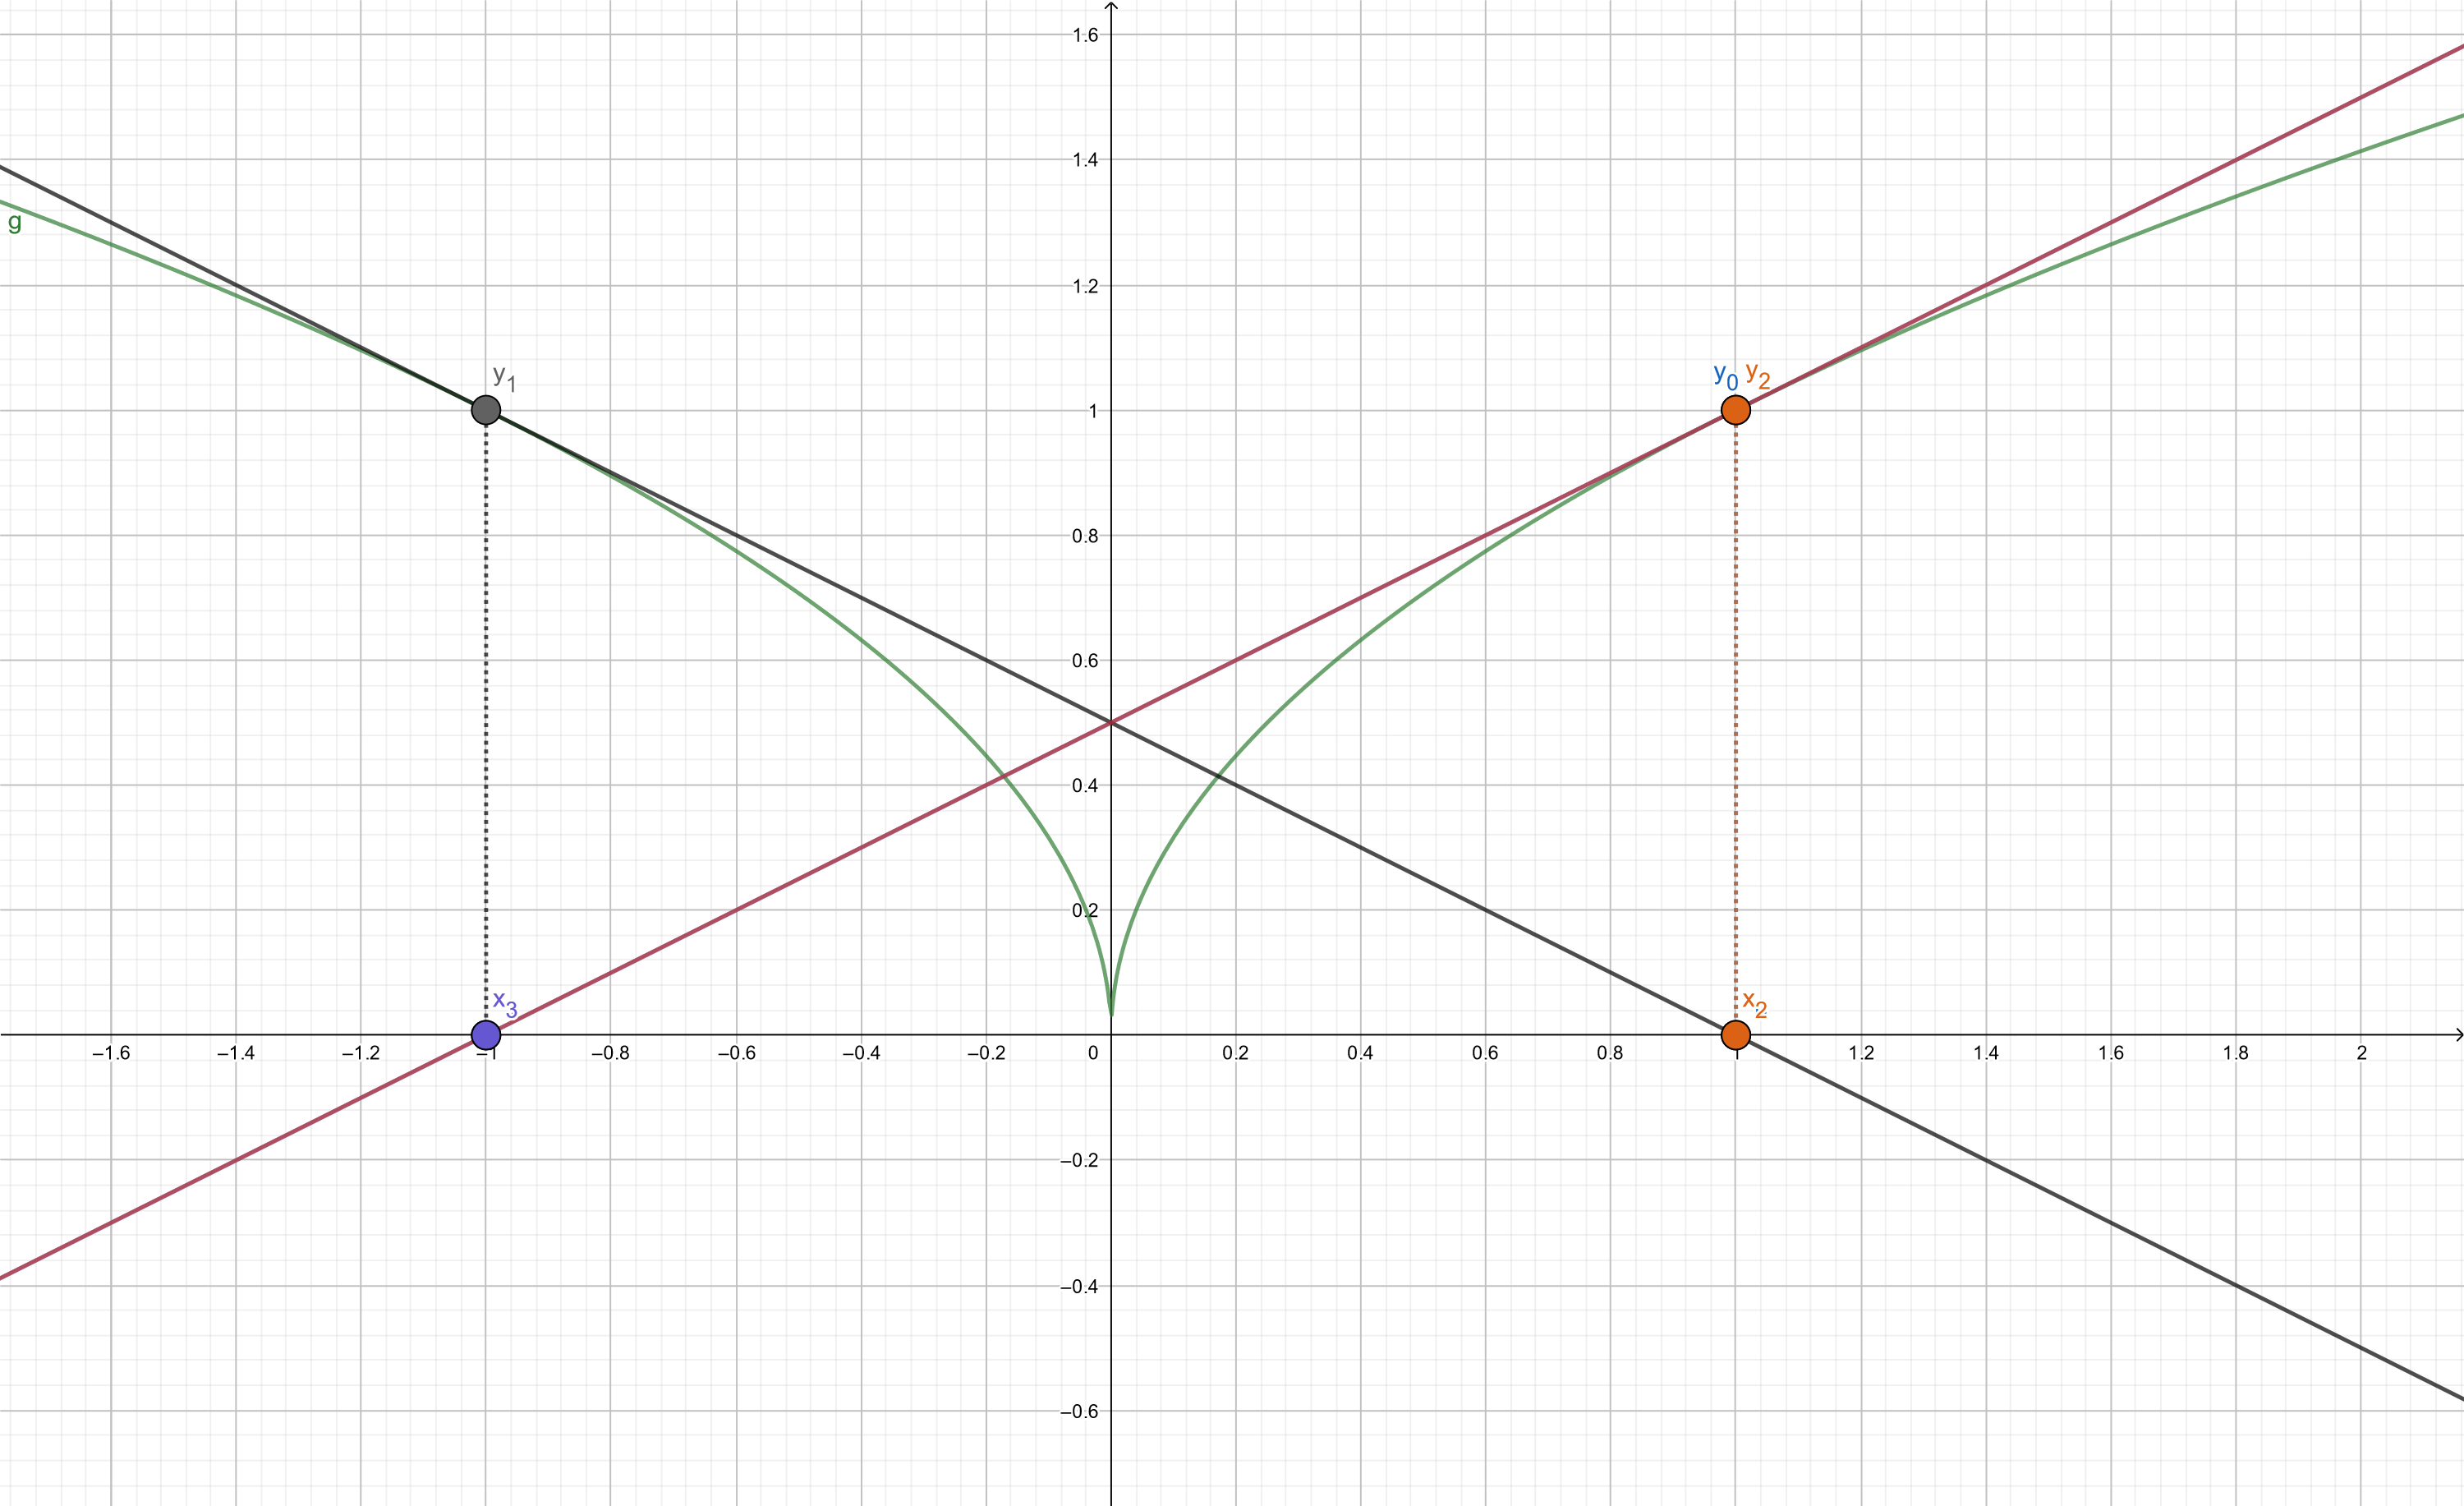
\includegraphics[width = 0.3\textwidth]{iteration-newton-2.png}
        \caption{Itérations de la méthode de Newton-Raphson pour $g(x) = \lvert x \rvert ^{\frac12}$ telle que $x_0 = 1$}
        \label{fig:nr-iterations-2}
    \end{figure}
\end{exemple}

\subsubsection{Cas de convergence lente $f:\mathbb{R}\rightarrow \mathbb{R}$}
Lorsqu'une racine est au moins de multiplicité 2, alors la convergence n'est plus d'ordre quadratique mais presque linéaire. Cependant, si cette multiplicité est connue, il est possible de modifier la méthode pour retrouver une convergence quadratique locale. En notant $m$ cette mutiplicité, on obtient :
% TODO : Jacobien ? 
\begin{equation*}
    x_{n+1}=x_{n}-m\frac{f(x_{n})}{f'(x_{n})}
\end{equation*}

\begin{rmk}
    S'il existe deux racines, proches l'une de l'autre, l'algorithme aura besoin de plusieurs itérations pour s'approcher de l'une d'entre elles.
\end{rmk}

\subsubsection{Coût de la méthode}
Le coût de calcul de la méthode de Newton est important. En effet, à chaque itération, il est nécessaire d’évaluer la jacobienne de $f$. Or, cette évaluation est relativement coûteuse.

\subsection{Application à un problème d'optimisation mono-objectif libre}
La recherche de l'optimum d'une fonction s'apparente à la recherche des zéros de son gradient.
Soit le problème d'optimisation, avec $f:\Omega \subset \mathbb{R}^n \rightarrow \mathbb{R}$
\begin{equation}
    (\mathscr{P}):\quad\min_{x\in \Omega} f(x)
    \label{eq:probleme-opt}
\end{equation}
La méthode de Newton-Raphson peut donc être appliquée au problème d'optimisation (\ref{eq:probleme-opt}) en choisissant $g(x)=\nabla f(x)$.
\begin{thm}
    Soit une fonction $f:\Omega \in \mathbb{R}^n\rightarrow \mathbb{R}$, deux fois différentiable, strictement convexe et de hessienne K-lipschitzienne dans un voisinage de $x_*$. Soit une valeur initiale $x_0\in Omega$, alors la suite $(x_k)_{k\in \mathbb{N}}$ définie par
    \begin{equation}
        x_{k+1}=x_k-\nabla^{2}f(x_k)^{-1}\cdot \nabla f(x_k)
        \label{eq:nr-opt-mono}
    \end{equation}
    converge quadratiquement vers $x_*$, le minimum de $f$, dans son voisinage.
\end{thm}

\begin{rmk}
    Si $f$ n'est pas de hessienne K-lipschitzienne, la convergence de la méthode de Newton-Raphson est superlinéaire.
\end{rmk}

\subsubsection{Convergence restreinte au voisinage de $x_*$}
Encore une fois, l'intérêt de la méthode de Newton-Raphson est limitée par la restriction sur la valeur initiale $x_0$ qui doit être dans un voisinage de $x_*$.
Ce problème peut être résolu en ajoutant une phase de recherche linéaire dans la direction
\begin{equation*}
    d_{k} = -\nabla ^{2}f(x_{k})^{-1} \nabla f(x_{k})
\end{equation*}
telle que la suite $(x_k)_{k\in \mathbb{N}}$ soit définie par
\begin{equation}
    x_{k+1}=x_k+t_k\cdot d_k
    \label{eq:nr-opt-mono-avec-line-search}
\end{equation}
avec $t_k$ le pas résultant d'une recherche linéaire.
Compte tenu des propriétés choisies pour $f$, $d_k$ est une direction de descente en $x_k$. En effet, la stricte convexité de $f$ implique que la hessienne soit strictement définie positive.
\begin{rmk}
    Si la stricte convexité de $f$ n'est pas vérifiée, il faudra vérifier que la hessienne est strictement définie positive. Ce résultat n'est pas garanti. S'il existe une solution au problème, on sait tout au plus que $\nabla^2f(x_*)>0$.
\end{rmk}

\subsubsection{Optima locaux}
L'application de la méthode de Newton à des fonctions non convexes est limitée par la non différentiation entre les différents points stationnaires. Dans le général, où $f$ est une fonction deux fois différentiable, la convergence de la méthode de Newton-Raphson n'implique pas l'obtention d'un minimum global de $f$, particulièrement si la valeur initiale $x_0$ est mal choisie. La fonction peut posséder plusieurs minima. Pour pallier à ce problème, différents solutions existent. Parmi elles, des méthodes hybrides (utilisation d'un algorithme génétique en parallèle de la méthode) ont été développé.

La méthode \textit{Hybrid Genetic Deflated Newton} (HGBN) \cite{art:Noack_Funke_2017} est particulièrement équipée pour optimiser des fonctions qui possède de nombreux optima locaux. Elle consiste en l'application locale de multiples algorithmes de Newton-Raphson sur une population d'individus - les valeurs initiales - pour identifier des optima et les rendre introuvable ($deflation$). La nouvelle génération est sélectionnée par survie du plus adapté, et on recherche de nouveau les optima jusqu'à les avoir tous trouvé.

HGBN converge vers un optimum global, et réduit significativement le nombre d'évaluations de fonctions nécessaire.

\begin{rmk}
    Concernant la recherche d'un optimum global, une alternative raisonnable serait la méthode du recuit simulé (\textit{simulated annealing} en anglais). Sur des problèmes où l'optimum global est enfoui parmi de multiples optima locaux, le recours à cette méthode est un choix raisonnable, quitte à être contraint à paramétrer l'algorithme manuellement, étant donné que c'est une méthode métaheuristique.
\end{rmk}

\subsubsection{Nombre d'évaluations, de calcul}
Les itérations de la méthode de Newton-Raphson nécessite l'évaluation du gradient, et de l'inverse de la hessienne de $f$ (matrice de taille $n\times n$). Dépendant de l'implémentation de l'algorithme, l'inversion de la hessienne de $f$ est également à prendre en compte, e.g. si on décide de ne pas l'inverser manuellement. La méthode de Newton-Raphson est donc informatiquement coûteuse, l'inversion d'une matrice étant souvent implémentée par la résolution d'un système d'équations linéaires.

\subsubsection{Propriétés de $f$}
La méthode de Newton-Raphson est valable si certaines propriétés de $f$ sont vérifiées : stricte convexité, deux fois différentiable. Cela restreint considérablement le champ d'application de la méthode de Newton-Raphson.

Si la fonction $f$ est seulement convexe, la hessienne de $f$ est semi-définie positive. Elle n'est donc pas forcément inversible.

\subsubsection{Vers les méthodes de quasi-Newton}
La nécessité que $f$ soit deux fois différentiable, et strictement convexe, ainsi que le coût relativement élevé de calcul des itérations de la méthode de Newton-Raphson est une faiblesse majeure de l'algorithme.

Cependant, les méthodes à métrique variable introduisent l'idée d'approximer l'inverse de la hessienne pour réduire à la fois les restrictions placées sur $f$, et réduire les coûts de calcul.

\section{Méthode de BFGS}

\subsection{Origines}
La méthode de Davidon (1959)\cite{art:Davidon_1991} qu'il nomme lui-même méthode à métrique variable est la base de nombreux travaux. Cette méthode de résolution de problèmes d'optimisation non-linéaire libre a la particularité de considérer une matrice variable d'une itération à une autre, i.e. la matrice $B$ estimation de l'inverse de la hessienne. Parmi les mathématiciens s'étant penché sur ces travaux, Fletcher et Powell proposent en 1963 une variation de la méthode à métrique variable (formule de DFP), dont Broyden louera les nombreuses qualités en 1970, en la comparant à ses travaux précédent. Il s'avance même en qualifiant à l'époque la méthode DFP de meilleur algorithme pour résoudre un problème d'optimisation libre, où l'expression explicite du gradient est accessible. En 1967, Broyden décrit la classe d'algorithmes qu'il nomme les méthodes de Quasi-Newton \cite{art:Broyden_1967}, généralisation de la méthode de la sécante dans le cas multidimensionnel basée sur les travaux de Wolfe (1659) et de Barnes (1965). En 1970, Broyden, Fletcher, Goldfarb et Shanno proposent le dual de la formule de DFP : la formule de BFGS, qui partage les caractéristique de la formule de DFP, mais donne de meilleurs résultats en pratique.
\begin{rmk}
    Fletcher détaille les caractéristiques des méthodes de la famille Broyden dans son ouvrage d'optimisation \cite{book:Fletcher_1987}, parmi lesquelles on retrouve la formule de DFP, de BFGS, et également la formule de Broyden, qui fût découverte après la formule de DFP, mais dont l'intérêt était diminué par ses inconvénients.
\end{rmk}

\subsection{Principe}
Dans cette partie, on considère le problème \ref{eq:probleme-opt}, avec $f:\Omega\subset \mathbb{R}^n\rightarrow \mathbb{R}$, une fonction une fois différentiable et convexe. Les méthodes de quasi-Newton se reposent sur l'approximation quadratique au voisinage de la solution, qui est le principe fondamental de la méthode de Newton.

La différence principale se situe dans la direction de descente de l'algorithme. \`A la place de la hessienne (resp. l'inverse de la hessienne) de $f$, on considèrera son approximation, notée $B$ (resp. $H$).\footnote{La notation est l'opposée de celle utilisée dans le polycopié de S. Mottelet \cite{poly:mottelet2003}, mais on choisit la convention employée par Fletcher dans \cite{book:Fletcher_1987}}

\subsubsection{Méthodes de quasi-Newton}
\begin{definition}
    Soit une itération $k$ de la méthode de Newton-Raphson, on considère un modèle approximatif quadratique $\varphi$\footnote{Dans le polycopié de RO04, S. Mottelet \cite{poly:mottelet2003} considère la notation $\varphi(t) = f(x+td)$.} de $f$ au voisinage de $x_{k}$ définie par
    \begin{align}
        \varphi_k(x) := f(x_k) & + \nabla f(x_k) (x - x_k)\nonumber \\
                               & + \frac12 (x-x_k)^T B_k (x-x_k)
        \label{eq:modele-quadra-qn}
    \end{align}
\end{definition}

\begin{definition}
    Incluant une phase de recherche linéaire, l'expression de la suite $(x_k)_{k\in \mathbb{N}}$ et sa direction de descente $d_k$ est définie par
    \begin{align}
        d_k = -B_k^{-1}\cdot \nabla f(x_k)\nonumber \\
        x_{k+1} = x_k + t_k\cdot d_k
        \label{eq:suite-qn}
    \end{align}
\end{definition}

\begin{pf}
    La direction de descente de quasi-Newton $d_k$ est définie comme le minimum du modèle quadratique de $f$ en $x_k$. Le gradient de $\varphi$ est calculé par rapport à $(x - x_k)$.
    \begin{align*}
        \nabla \varphi_k(x) & =\nabla f(x_k) + B_k(x-x_k)                      \\
                            & = x_k \underbrace{- B_k^{-1}\nabla f(x_k)}_{d_k}
    \end{align*}
    La formule de mise à jour finale est obtenue en considérant une phase de recherche linéaire de pas noté $t_k$ :
    \begin{equation}
        d_k = -B_k\cdot g_k \\
        x_{k+1} = x_k + t_k\cdot d_k
    \end{equation}
\end{pf}

\begin{rmk}
    L'expression de la direction de descente $d_k$ pour la matrice $H$ peut être obtenue en remplaçant $B_k$ par $H_k^{-1}$ dans $\varphi$.
\end{rmk}
\begin{rmk}
    Les directions de descente de quasi-Newton successives sont conjuguées.
\end{rmk}

\begin{definition}
    Soit l'équation de la sécante, ou condition de quasi-Newton définie par
    \begin{align}
        y_k = B_{k+1} \cdot s_k
        \label{eq:sec-qn-bk} \\
        H_{k+1} \cdot y_k = s_k
        \label{eq:sec-qn-hk} \\
    \end{align}
    avec $y_k = \nabla f(x_{k+1}) - \nabla f(x_k)$ et $s_k = x_{k+1} - x_k$.
\end{definition}
\begin{pf}
    On impose à la mise à jour de l'approximation quadratique $\varphi_{k+1}$ l'égalité des gradients en $x_k$ et $x_{k+1}$.
    Vérifions la première condition.
    \begin{align*}
        \nabla \varphi_{k+1}(x_{k+1}) & = \nabla f(x_{k+1}) + B_{k+1}(x_{k+1} - x_{k+1}) \\
                                      & = \nabla f(x_{k+1})                              \\
    \end{align*}
    Vérifions la deuxième condition.
    \begin{align*}
             & \nabla \varphi_{k+1}(x_{k}) = \nabla f(x_{k+1}) - B_{k+1}s_k \\
        \iff & y_k = B_{k+1}\cdot s_k
    \end{align*}
\end{pf}

\begin{rmk}
    L'équation de la sécante ici définie montre bien la raison pour laquelle on considère les méthodes de quasi-Newton comme une généralisation multidimensionnelle de la méthode de la sécante.
\end{rmk}
\begin{definition}
    Soit les valeurs initiales $x_0\in \Omega$, $B_0$ ou $H_0$. Une méthode de quasi-Newton est une méthode à métrique variable dont la suite $(x_k)_{k\in \mathbb{N}}$ est définie par
    \begin{align*}
         & d_k = -B_k^{-1}\cdot \nabla f(x_k) = -H_k\cdot \nabla f(x_k) \\
         & x_{k+1} = x_k + t_k\cdot d_k
    \end{align*}
    et les formules de mise à jour de $B_k$ et $H_k$
    \begin{align}
        B_{k+1} = B_k + \Delta_k
        \label{eq:maj-bk} \\
        H_{k+1} = H_k + \Delta_k
        \label{eq:maj-hk}
    \end{align}
    vérifient l'équation de la sécante, où $\Delta_k$ correspond à une matrice symétrique de rang connu tel que les conditions de quasi-Newton soient vérifiées.
\end{definition}

\begin{definition}
    Soit $\Delta_k$ une matrice symétrique de rang $i$, on dit que la formule de mise à jour de $B_k$ ou $H_k$ correspondante est une formule de correction de rang $i$.
\end{definition}

\subsubsection{Faiblesses des méthodes de quasi-Newton}
L'efficacité des méthodes de quasi-Newton repose sur la positivité de la matrice approximation au cours des itérations de l'algorithme. Broyden a nommé cette propriété la stabilité d'une méthode de quasi-Newton. En effet, il faut conserver la direction de descente $d_k$ au cours des itérations. Ainsi, une formule de mise à jour est d'autant meilleure qu'elle préserve la positivité de la matrice initiale. \`A cette fin, on définit une condition dite condition de courbure équivalente à la positivité de la matrice approximation.

\begin{definition}
    On appelle la condition de courbure l'inéquation
    \begin{equation}
        s^ky_k > 0
    \end{equation}
\end{definition}
\begin{pf}
    La condition de courbure est obtenue en multipliant à gauche (\ref{eq:sec-qn-bk}) ou (\ref{eq:sec-qn-hk}).
\end{pf}
\begin{rmk}
    La condition de courbure est vérifiée lorsqu'une méthode de recherche linéaire inexacte est employée \cite{poly:mottelet2003}.
\end{rmk}

Aussi, les itérations de l'algorithme dépendant de la nature inversible de la matrice approximation, il faut également conserver cette caractéristique. Si la matrice venait à devenir non inversible lors d'une mise à jour, alors la méthode devra s'arrêter.

La condition de quasi-Newton nous montre qu'il existe une infinité de matrices approximations la vérifiant. En effet, c'est un système de $n$ équations linéaires à $\frac{n(n+1)}{2}$ degrés de libertés. En effet, on considère ici toutes les composantes de la matrice approximation comme des variables libres. Cette matrice étant symétrique, il existe $\frac{n(n+1)}{2}$ paramètres ajustables.

\begin{rmk}
    La stabilité d'une méthode de quasi-Newton n'est pas suffisante pour prouver sa convergence.
\end{rmk}

\subsubsection{Formule de BFGS}
\begin{definition}
    La formule de mise à jour de Broyden, Fletcher, Goldfarb et Shanno, formule de correction de rang 2, est définie dans sa forme développée par
    \begin{align}
        H_{k+1} = H_k & + \left(I + \frac{y_k H_k y_k}{s_k^T y_k}\right)\frac{s_k s_k^T}{s_k^T y_k}\nonumber \\
                      & -\left(\frac{s_k y_k^T H+ H y_k s_k^T}{s_k^T y_k}\right)
        \label{eq:bfgs-hk-developed}
    \end{align}
    On peut factoriser cette expression comme suit
    \begin{equation}
        H_{k+1} = \left(I - \frac{y_k s_k^T}{s_k^T y_k}\right) H_k \left(I - \frac{s_k y_k^T}{s_k^Ty_k}\right) + \frac{y_k y_k^T}{s_k^T y_k}
        \label{eq:bfgs-hk-factorised}
    \end{equation}
    La formule de mise à jour de $H_k$ permet d'obtenir celle de $B_{k}$
    \begin{equation}
        B_{k+1} = B_k + \frac{y_ky_k^T}{y_k^Ts_k}-\frac{B_ks_ks_k^TB_k}{s_k^TB_ks_k}
        \label{eq:bfgs-bk}
    \end{equation}
\end{definition}

La formule de DFP met à jour la matrice $H_k$ en contraignant les itérations suivantes à vérifier (\ref{eq:sec-qn-hk}). L'idée derrière la formule de BFGS est de proposer un pendant en forçant les itérations à vérifier (\ref{eq:sec-qn-bk}) en considérant $B_{k+1} = H_{k+1}^{-1}$. En échangeant $y_k$ et $s_k$, on obtient une nouvelle formule de mise à jour pour $H_{k+1}$.

La formule de BFGS est donc obtenue à partir de la formule de DFP et partage nombreuses de ses propriétés.
\begin{rmk}
    On préfère la formule de mise à jour de $B_{k+1}$ au lieu de son inverse $H_{k+1}$, car cette dernière a un défaut significatif. En effet, la mise à jour de $H_{k+1}$ est sensible aux arrondis de calcul, et on risque de perdre la positivité de la matrice. Malgré que le nombre d'opérations nécessaire soit supérieur, cette différence peut être palliée par la factorisation $LDL^T$ de la matrice $B_{k}$. Le nombre d'opérations nécessaire à la mise à jour devient alors sensiblement identique à celui pour mettre à jour $H_{k+1}$ \cite{book:GillMurrayWright1981}.
\end{rmk}

\begin{thm}
    Si $s_k^Ty_k > 0, \forall k$, alors la positivité de la matrice $B_{k}$ est préservée au cours des itérations.
\end{thm}

Ce théorème est sans doute le plus important de cette section, car en d'autres mots, la méthode de quasi-Newton équipée de la formule de BFGS "progresse" toujours à chaque itération. Autrement dit, la direction de descente $d_k$ reste une direction de descente au cours des itérations de la méthode.

Aussi, les imprécisions de la recherche linéaire affectent sensiblement moins l'algorithme,

\begin{thm}
    Soit $B_0$, une matrice initiale symétrique définie positive et une valeur initiale $x_0\in\Omega$. Soit $f$ une fonction différentiable, convexe, et de gradient $K$-Lipschizien. La suite $(x_k)_{k\in \mathbb{N}}$ générée par la méthode de quasi-Newton avec la formule de BFGS et équipée d'une méthode de recherche linéaire converge superlinéairement vers la solution $x_*$ du problème (\ref{eq:probleme-opt}).
\end{thm}
\begin{pf}
    La convergence globale de la méthode de BFGS avec l'utilisation d'une méthode de recherche linéaire inexacte a été prouvée dans les travaux de Fletcher. \cite{book:Fletcher_1987}.
\end{pf}

\begin{rmk}
    Le calcul du pas optimal $\hat t$ pour la méthode de quasi-Newton avec la formule de BFGS implique la terminaison de l'algorithme en au plus $n$ itérations \cite{book:Fletcher_1987}.
\end{rmk}

Comparée à la formule de DFP, la formule de BFGS donne à l'algorithme de quasi-Newton une plus grande résistance aux imprécisions dû à l'approximation de la hessienne (ou son inverse). Ainsi, le risque de rendre la matrice approximation non inversible est moindre.

C'est pour ces raisons que l'on préfèrera l'utilisation de la formule de BFGS, que beaucoup considèrent comme la meilleure méthode d'optimisation libre sans contraintes.

Bien que la vitesse de convergence des méthodes de quasi-Newton soit en général inférieure à celle de la méthode de Newton-Raphson, elles ont une complexité calculatoire bien inférieure, car la hessienne n'est pas évaluée.

\subsection{Algorithme de Broyden, Fletcher, Goldfarb et Shanno dit BFGS}
Soit une valeur initiale $x_0$, une matrice symétrique définie positive $H_0$, de préférence une estimation raisonnable ou par défaut la matrice identité $I$.
\begin{enumerate}
    \item \`A l'itération $k$, la direction de descente est calculée selon
          \begin{equation*}
              d_{k}=-B_{k}^{-1}\nabla f(x_{k})
          \end{equation*}
    \item Ensuite, le pas optimal $\hat t$ est calculé, ou une méthode de recherche linéaire inexacte est utilisée pour déterminer le pas $t_k$. On calcule ensuite l'itéré suivant :
          \begin{equation*}
              x_{k+1}=x_{k}+\rho_{k}d_{k}
          \end{equation*}
    \item On met à jour la matrice $B_{k}$ ou $H_{k}$.
    \item L'algorithme continue, sauf si le ou les critères d'arrêts spécifiés sont vérifiés.
\end{enumerate}

La matrice $H_{k}$ étant symétrique définie positive, elle peut être décomposée en deux matrices triangulaires par la décomposition de Chloesky. Ainsi, en posant $H_{k}=C_{k}C_{k}^{T}$, la mise à jour de la matrice $H_{k}$ devient moins coûteuse, plus précisement de même complexité que pour la formule de DFP.

Plus loin, on propose d'autres méthodes de factorisation de Cholesky. Ces techniques permettent d'éviter des erreurs d'arrondis, grâce à un contrôle plus précis du caractère défini positif de la matrice $H_{k}$.

\begin{rmk}
    \textbf{Convergence de $(B_k)_{k\in \mathbb{N}}$} - La formule de BFGS est qualifiée de formule de moindres changements (\textit{least changes update formula}), c'est-à-dire qu'on cherche à effectuer le moins de changements possibles sur la matrice $B_k$. Pour les formules de moindres changements, la suite $(B_k)_{k\in \mathbb{N}}$ converge vers l'inverse de la hessienne. Ce n'est pas forcément le cas pour toutes les formules de mise à jour.
\end{rmk}

\subsubsection{Variation de la méthode de BFGS : L-BFGS}
La méthode L-BFGS (Limited-memory BFGS) est une variation de la méthode de BFGS qui ne stocke pas entièrement la matrice $H_k$. De cette manière, la direction de descente n'est pas calculée directement à partir de la matrice $H_k$, mais en faisant usage d'un historique des mises à jours effectuées. La complexité calculatoire et de stockage devient ainsi linéaire, proportionnelle à la taille de l'historique des mises à jours.

\section{Implémentation}
Toutes les implémentations des algorithmes suivants ont été réalisé sur SCILAB 6.1.0.\footnote{https://www.scilab.org/}.

On souhaite tout d'abord définir les algorithmes supports qui nous serviront par la suite. Ainsi, on s'intéressa premièrement aux méthodes de recherche linéaire inexacte, puis à la factorisation de Cholesky.

\subsection{Recherche linéaire inexacte}
Contrairement au calcul d'un pas $\hat t$ exact (optimal), la recherche linéaire inexacte fait usage d'un intervalle de sécurité pour lequel on qualifie le pas $t$ de convenable, ou au contraire trop petit ou trop grand. On cherche ainsi à assurer une décroissance suffisante dans une direction de descente donnée. Il existe plusieurs règles caractérisant la réduction de l'intervalle de sécurité. Parmi elles, on s'intéresse aux règles d'Armijo, Golstein et Wolfe-Powell.

On note $f$ la fonction à optimiser, $\nabla f$ l'expression de son gradient, $x_k$ une itération de l'algorithme d'optimisation, $d_k$ la direction de descente de l'itération $k$, et $\varphi$ une fonction du pas $t$ définie par $\varphi(t)=f(x_k+td_k)$. On définit $I=[\alpha,\beta]$, l'intervalle de sécurité contenant le pas $t$.

\begin{rmk}
    Avec la notation utilisée, $\varphi'(0)=\nabla f(x_k)^T d_k$.
\end{rmk}
\subsubsection{Règle d'Armijo}
\begin{definition}
    Soit un réel $m$ compris strictement entre $0$ et $1$. On définit l'intervalle de sécurité par $I=[0,\beta]$. La règle d'Armijo est définie par la condition suivante
    \begin{equation}
        \varphi(t) \leq \varphi(0) + m\varphi'(0)t
        \label{eq:armijo}
    \end{equation}
    Si la condition d'Armijo est vérifiée, alors on dit que le pas $t$ convient. Sinon, le pas $t$ est trop grand.
\end{definition}
La règle d'Armijo ne définit une restriction que si le pas est trop grand.

\subsubsection{Règle de Goldstein}
La règle de Goldstein rajoute une condition sur la petitesse du pas $t$ à la règle d'Armijo.
\begin{definition}
    Soit deux réels $m_1$, et $m_2$ vérifiant $0<m_1<m_2<1$. On définit l'intervalle de sécurité $I$ par $I=[\alpha,\beta]$. La règle de Goldstein est définie par les conditions suivantes
    \begin{align}
        \varphi(t) \leq \varphi(0) + m_1\varphi'(0)t
        \label{eq:goldstein-grand} \\
        \varphi(t) \geq \varphi(0) + m_2\varphi'(0)t
        \label{eq:goldstein-petit}
    \end{align}
    Si les conditions de Goldstein sont vérifiées, on dit que le pas $t$ convient. Sinon, si (\ref{eq:goldstein-grand}) n'est pas vérifiée, on dit que le pas $t$ est trop grand. Si (\ref{eq:goldstein-petit}) n'est pas vérifiée, on dit que le pas $t$ est trop petit.
\end{definition}
\begin{rmk}
    Dans la pratique, on choisit $m_1=0.1$ et $m_2 = 0.7$. Par ailleurs, le choix de $m_2$ est préférable tel que $m_2\geq \frac12$, de sorte à ce que le pas optimal soit inclus dans l'intervalle de sécurité.
\end{rmk}
\subsubsection{Règle de Wolfe-Powell}
La règle de Wolfe-Powell rajoute à la règle d'Armijo une condition sur la dérivée $\varphi'(t)$, qui permettra par la suite de réduire $I$ par une méthode d'interpolation cubique.
\begin{definition}
    Soit deux réels $m_1$, et $m_2$ vérifiant $0<m_1<m_2<1$. On définit l'intervalle de sécurité $I$ par $I=[\alpha,\beta]$. La règle de Wolfe-Powell est définie par les conditions suivantes
    \begin{align}
        \varphi(t)  & \leq \varphi(0) + m_1\varphi'(0)t
        \label{eq:wolfe-powell-grand}                   \\
        \varphi'(t) & \geq m_2\varphi'(0)t
        \label{eq:wolfe-powell-petit}
    \end{align}
    Si les conditions de Wolfe-Powell sont vérifiées, on dit que le pas $t$ convient. Sinon, si (\ref{eq:wolfe-powell-grand}) n'est pas vérifiée, on dit que le pas $t$ est trop grand. Si (\ref{eq:wolfe-powell-petit}) n'est pas vérifiée, on dit que le pas $t$ est trop petit.
\end{definition}
La règle de Wolfe-Powell garantit que le pas $t$ n'est pas trop petit en s'assurant que la pente après descente $\varphi'(t)$ a suffisamment augmenté.
\begin{rmk}
    $\varphi'(t) = \nabla f(x_k+td_k)^Td_k$.
\end{rmk}
L'algorithme de recherche linéaire inexacte est découpée en plusieurs phases : la recherche d'un intervalle de départ, puis la réduction de l'intervalle, soit par dichotomie, soit par une approximation cubique de $\varphi(t)$ lorqu'on utilise la règle de Wolfe-Powell.

\begin{rmk}
    Dans l'algorithme~(\ref{algo:line-search}), la règle utilisée n'est pas explicitée, mais sont utilisées les conditions "$t$ est trop petit", "$t$ est trop grand", ou "$t$ convient".
\end{rmk}
\begin{algorithm}[ht]
    \centering{
        \fbox{
            \begin{minipage}[t]{150mm}
                \footnotesize
                \renewcommand{\baselinestretch}{2.5}
                \resetline
                \begin{tabbing}
                    aaaA\=aA\=aaaA\=aaA\=aaA\=aaA\=aaA\kill
                    {\bf  Entrée :}\\
                    \> $f$ \>:= la fonction à optimiser\\
                    \> $\nabla f$ \>:= l'expression analytique du gradient de $f$\\
                    \> $x_k$ \> := l'itération $k$\\
                    \> $d_k$ \> := la direction de descente associée\\
                    \> $t$ \> := une valeur initiale du pas\\
                    \> $m_1$ \> := paramètre d'ajustement de $\alpha$\\
                    \> $m_2$ \> := paramètre d'ajustement de $\beta$\\
                    \> $c$ \> := paramètre d'ajustement de la recherche d'un\\ \>\> intervalle de départ $I$, $c>1$\\
                    {\bf  Sortie :}\\
                    \> $t$ \> := le pas choisi\\
                    {\bf  Initialisation :}\\
                    \line{LINE-01} \> $m_1$ \>: si la valeur n'a pas été précisée, $m_1=0.1$\\
                    \line{LINE-02} \> $m_2$ \>: si la valeur n'a pas été précisée, $m_2=0.7$\\
                    \line{LINE-03} \> $c$ \>: si la valeur n'a pas été précisée, $c=2$\\
                    \line{LINE-04} \> $\alpha$ \>:= la borne inférieure de $I$, $\alpha=0$\\
                    \line{LINE-05} \> $\beta$ \>:= la borne supérieure de $I$\\
                    {\bf Recherche d'un intervalle de départ $I$ :}\\
                    \line{LINE-06} \> {\bf Si} $t$ convient, {\bf alors} l'algorithme (\ref{algo:line-search}) s'arrête.\\
                    \line{LINE-07} \> {\bf Sinon si} $t$ est trop grand, {\bf alors} $\beta=t$.\\
                    \line{LINE-08} \> {\bf Sinon faire :}\\
                    \line{LINE-09} \>\>{\bf Tant que} $t$ est trop petit {\bf faire :}\\
                    \line{LINE-10} \>\>\> $t=c\cdot t$\\
                    \line{LINE-11} \>\> {\bf Si} $t$ convient, {\bf alors} l'algorithme (\ref{algo:line-search}) s'arrête.\\
                    \line{LINE-12} \>\> {\bf Si} $t$ est trop grand, {\bf alors} $\beta=t$.\\
                    {\bf Réduction de l'intervalle $I$ :}\\
                    \line{LINE-15} \> {\bf Tant que } $t$ ne convient pas {\bf faire :}\\
                    \line{LINE-16} \>\> $t=\frac{\alpha+\beta}{2}$ ou\\
                    \>\> $t_{\texttt{WP}} = \underset{t}\min$ {\texttt{INTERPOLATION$^3$}$_{\varphi}$}($t$, $\alpha$, $\beta$, $f$, $\nabla f$, $x_k$, $d_k$)\\
                    \line{LINE-17} \>\> {\bf Si } $t$ est trop petit {\bf alors} $\alpha=t$\\
                    \line{LINE-18} \>\> {\bf Sinon si} $t$ est trop grand {\bf alors} $\beta=t$\\
                    %------------------
                \end{tabbing}
                \normalsize
            \end{minipage}
        }
        \medbreak
        \caption{Algorithme de recherche linéaire inexacte}
        \label{algo:line-search}
    }
\end{algorithm}

\subsubsection{Interpolation cubique de $\varphi$}
On définit le minimum $t_{\min}$ de l'interpolation cubique de $\varphi$ par 
\[t_{\min} = \underset{t}\min\, \textrm{\texttt{INTERPOLATION}}^3_{\varphi}\left(t_0, \alpha, \beta, f, \nabla f, x_k, d_k\right)\]
 en prenant les notations de \cite{poly:mottelet2003}
\begin{align*}
    \varphi(t) &= f(x_k+td_k)\\
    \varphi'(t) &= \nabla f(x_k+td_k)^Td_k\\
    \tau &= \beta-\alpha\\
    a &= \tau(\varphi'(\alpha)+\varphi'(\beta))+2(\varphi(\alpha)-\varphi(\beta))\\
    b &= 3(\varphi(\beta)-\varphi(\alpha))-\tau(2\varphi'(\alpha)+\varphi'(\beta))\\
    c &= \tau\varphi'(\alpha)
\end{align*}
Si $b^2-3ac \geq 0$, alors il existe un minimum tel que 
\begin{equation}
    t_{\min} = t_0 + \tau\frac{-b+\sqrt{b^2-3ac}}{3a}
    \label{eq:min-interp-3}
\end{equation}
\subsubsection{Conditions d'arrêts et précision}
La recherche linéaire ne s'arrête pas tant qu'elle n'a pas trouvé de pas $t$ qui convienne. Cette méthode de recherche est inexacte, et le pas n'est pas optimal, mais on gagne en complexité calculatoire. Au lieu de calculer le pas optimal, on se contente de l'approcher, et cette approximation est suffisante pour que la méthode de quasi-Newton avec la formule de BFGS converge, ce qui n'est pas le cas pour la formule de DFP.

On préfèrera la règle de Wolfe-Powell, pour augmenter la vitesse de réduction de l'intervalle, qui n'est pas suffisante en utilisant une dichotomie simple. Cependant, si l'interpolation cubique ne donne n'est pas utilisable (soit car elle ne renvoie pas de minimum, soit car on n'utilise pas la règle de Wolfe-Powell), on peut se retrancher sur la dichotomie.

\subsubsection{Difficultées techniques}
L'implémentation de l'algorithme (\ref{algo:line-search}) n'est pas difficile. S'il y a un point à souligner lors de l'implémentation, c'est de faire attention à optimiser la vérification de la règle utilisée. Il faut à tout prix éviter de vérifier plusieurs fois de suite la même inégalité, au risque de ralentir la recherche. On pourra à cette fin stocker le résultat d'une comparaison dans une variable booléenne et en faire usage si nécessaire plus loin.

\subsection{Factorisation matricielle : factorisation $LDL^T$ de Cholesky}
L'implémentation d'une méthode de quasi-Newton requiert la mise à jour d'une matrice symétrique définie positive à chaque itération. Il est clair que la mise à jour d'une matrice entière avec de telles propriétés n'est pas une opération entièrement optimisé. Pour des raisons de performance, on préfèrera donc mettre à jour les facteurs d'une décomposition de la matrice $B_{k+1}$, issues de la factorisation alternative de Cholesky. L'algorithme modifié de Cholesky ici décrit est celui défini dans \cite{art:McSweeney_2017}.

\begin{rmk}
    On choisit $a_{ij}$ comme la notation du coefficient de ligne $i$ et de colonne $i$ d'une matrice $A$.
\end{rmk}
\begin{algorithm}[ht]
    \centering{
        \fbox{
            \begin{minipage}[t]{150mm}
                \footnotesize
                \renewcommand{\baselinestretch}{2.5}
                \resetline
                \begin{tabbing}
                    aaaA\=aA\=aaaA\=aaA\=aaA\=aaA\=aaA\kill
                    {\bf  Entrée :}\\
                    \> $B$\>:= matrice symétrique définie positive à factoriser\\
                    {\bf  Sortie :}\\
                    \> $L$\>:= matrice triangulaire inférieure unité\\
                    \> $D$\>:= matrice diagonale définie positive\\
                    {\bf  Initialisation :}\\
                    \line{CLDL-01} \> $n$ \>:= taille de la matrice $B$\\
                    \line{CLDL-02} \> $L$ \>:= matrice de zéros de taille $n\times n$\\
                    \line{CLDL-03} \> $D$ \>:= matrice de zéros de taille $n\times n$\\
                    {\bf Itérations :}\\
                    \line{CLDL-04} \> {\bf Pour } $j=1,\dots,n$ {\bf faire :}\\
                    \line{CLDL-05} \>\> $d_{jj} = a_{jj}-\sum_{k=1}^{j-1}l_{jk}^2\cdot d_{kk}$\\
                    \line{CLDL-06} \>\> {\bf Pour } $i=j+1,\dots,n$ {\bf faire :}\\
                    \line{CLDL-07} \>\>\> $l_{ij} = \frac{1}{d_{jj}}\left(a_{ij}-\sum_{k=1}^{j-1}l_{ik}l_{jk}d_{kk}\right)$\\
                    %------------------
                \end{tabbing}
                \normalsize
            \end{minipage}
        }
        \medbreak
        \caption{Algorithme de la factorisation alternative de Cholesky}
        \label{algo:cldlt}
    }
\end{algorithm}
\subsubsection{Conditions d'arrêts et précision}
L'algorithme (\ref{algo:cldlt}) n'explicite pas de conditions d'arrêts. Il est destiné ici à factoriser une matrice symétrique définie positive provenant de la méthode de quasi-Newton avec la formule de BFGS, qui préserve la positivité de sa matrice $B_k$ au cours des itérations.

Néanmoins, des erreurs éventuelles peuvent provenir de deux sources différentes : la matrice $B$, variable d'entrée; et le calcul de $d_{jj}$. Si la matrice d'entrée $B$ n'est pas définie positive, l'algorithme ne fonctionnera pas. Aussi, si lors du calcul de $d_{jj}$, le coefficient venait à devenir nul, alors le calcul de $l_{ij}$ en serait impacté, et l'algorithme s'arrête. Cette deuxième source d'erreur est en réalité identique à la première. En effet, le coefficient $d_{jj}$ s'annule uniquement si la matrice $B$ n'est pas définie positive. La factorisation de Cholesky peut mettre à profit cette caractéristique, et servir d'algorithme de vérification de la positivité d'une matrice \cite{art:McSweeney_2017}.

\subsubsection{Difficultées techniques}
La factorisation de Cholesky n'est pas algorithmiquement complexe à implémenter. Les difficultées techniques proviennent de l'utilisation optimale des opérateurs vectoriels (e.g. \texttt{.*}, \texttt{'}) de Scilab dans le but d'améliorer les performances.

\subsection{Méthode de Newton-Raphson}
\begin{algorithm}[ht]
    \centering{
        \fbox{
            \begin{minipage}[t]{150mm}
                \footnotesize
                \renewcommand{\baselinestretch}{2.5}
                \resetline
                \begin{tabbing}
                    aaaA\=aaaaA\=aaA\=aaA\=aaA\=aaA\kill
                    {\bf  Entrée :} \\
                    \> $f$ \>:= la fonction dont on cherche les racines\\
                    \> $\nabla f$ \>:= l'expression analytique du gradient de $f$\\
                    \> $\nabla^2 f$ \>:= l'expression analytique de la hessienne \\\>\>de $f$\\
                    \> $x_0 \in \Omega$ \>:= la valeur initiale de recherche\\
                    \> $\varepsilon \in \mathbb{R}^+_*$ \>:= la marge d'erreur acceptable,\\ \>\>le critère d'arrêt\\
                    \> $N\in \mathbb{N}$ \>:= le nombre d'itérations maximales\\
                    {\bf  Sortie :}\\
                    \> $x_*$ \>:= le minimum de $f$ trouvé, si la méthode\\\>\> converge\\
                    {\bf  Initialisation :}\\
                    \line{NR-01} \> $k = 0$ \>:= le nombre d'itérations actuels\\
                    \line{NR-02} \> $t_0 = 1$ \>:= le pas initial de l'itération $k$, puis \\
                    déterminé par une méthode de recherche linéaire\\
                    \line{NR-03} \> $\varepsilon = 10^{-10}$, si une précision n'est pas précisée.\\
                    {\bf Itérations :}\\
                    \line{NR-04} \> {\bf Tant que} $\lVert \nabla f(x_k) \rVert > \varepsilon$ {\bf ET} $k < N$ {\bf faire :}\\
                    \line{NR-05} \>\> $d_k = -\nabla^2 f(x_k)^{-1}\cdot \nabla f(x_k)$\\ 
                    \line{NR-06} \>\> Choisir $t_k$ selon l'algorithme (\ref{algo:line-search})\\ 
                    \line{NR-07} \>\> $x_{k+1} = x_k + t_k d_k$\\
                    \line{NR-09} \>\> $k = k+1$\\
                    %------------------
                \end{tabbing}
                \normalsize
            \end{minipage}
        }
        \medbreak
        \caption{Algorithme de la méthode de Newton-Raphson}
        \label{algo:newton_raphson}
    }
\end{algorithm}
\subsubsection{Conditions d'arrêts et précision}
On définit deux conditions d'arrêts à l'algorithme (\ref{algo:newton_raphson}) : si la précision voulue est atteinte, ou si le nombre d'itérations maximal est dépassé. La première condition d'arrêt est nécessaire car l'algorithme ne s'arrêterait pas une fois qu'il se soit approché d'une racine de $\nabla f$. La deuxième condition d'arrêt est nécessaire et arrête l'algorithme lorsqu'il ne trouve rien. Cela peut arriver lorsqu'une itération se trouve sur un optimum de $f$, ou dans des situations particulières telles comme dans l'exemple (\ref{ex:newton-raphson-non-differentiable}).

La précision de l'algorithme de quasi-Newton dépend de l'entrée utilisateur.

\subsubsection{Difficultées techniques}
L'implémentation de l'algorithme de Newton-Raphson n'est pas difficile. Il n'y a presque aucune difficulté technique.

On fera néanmoins attention à l'inversion de $\nabla^2 f(x_k)$, qui se réalisera à travers une division matricielle gauche. L'opérateur utilisée sera \texttt{\textbackslash}. Cet opérateur est bien plus efficace que la commande d'inversion \texttt{inv}, qui résout le système d'équations linéaires \cite{doc:scilab-backslash}.

\subsection{Méthode de BFGS}
L'algorithme de la méthode de BFGS qu'on décrit ici, ne fait pas usage de la factorisation alternative de Cholesky décrit dans l'algorithme (\ref{algo:cldlt}) pour des raisons expliquées ci-après. Pour réduire la complexité calculatoire, on fera donc usage de la formule de mise à jour (\ref{eq:bfgs-hk-factorised}).

\begin{algorithm}[ht]
    \centering{
        \fbox{
            \begin{minipage}[t]{150mm}
                \footnotesize
                \renewcommand{\baselinestretch}{2.5}
                \resetline
                \begin{tabbing}
                    aaaA\=aaaaA\=aaA\=aaA\=aaA\=aaA\kill
                    {\bf  Entrée :} \\
                    \> $f$ \>:= la fonction qu'on cherche à optimiser\\
                    \> $\nabla f$ \>:= l'expression analytique du gradient de $f$\\
                    \> $x_0 \in \Omega$ \>:= la valeur initiale de recherche\\
                    \> $H_0 \in \Omega$ \>:= la matrice initiale \\
                    \> $\varepsilon \in \mathbb{R}^+_*$ \>:= la marge d'erreur acceptable,\\ \>\>le critère d'arrêt\\
                    \> $N\in \mathbb{N}$ \>:= le nombre d'itérations maximales\\
                    {\bf  Sortie :}\\
                    \> $x_*$ \>:= le minimum de $f$ trouvé, si la méthode\\\>\> converge\\
                    {\bf  Initialisation :}\\
                    \line{BFGS-01} \> $k = 0$ \>:= le nombre d'itérations actuels\\
                    \line{BFGS-02} \> $t_0 = 1$ \>:= le pas initial de l'itération $k$, puis \\
                    déterminé par une méthode de recherche linéaire\\
                    \line{BFGS-03} \> $H_0 = I$ \>:= si elle n'est pas définie \\
                    \line{BFGS-04} \> $\varepsilon = 10^{-10}$, si une précision n'est pas précisée.\\
                    {\bf Itérations :}\\
                    \line{BFGS-05} \> {\bf Tant que} $\lVert f(x_k) \rVert> \varepsilon$ {\bf ET} $k < N$ {\bf faire :}\\
                    \line{BFGS-06} \>\> $d_k = - H_{k}\cdot \nabla f(x_k)$\\
                    \line{BFGS-07} \>\> Choisir $t_k$ selon l'algorithme (\ref{algo:line-search})\\
                    \line{BFGS-08} \>\> $x_{k+1} = x_k + t_k d_k$\\
                    \line{BFGS-09} \>\> $s_k = t_k d_k$\\
                    \line{BFGS-10} \>\> $y_k = \nabla f(x_{k+1}) - \nabla f(x_k)$\\
                    \line{BFGS-11} \>\> $H_{k+1} = \left(I - \frac{y_k s_k^T}{s_k^T y_k}\right) H_k \left(I - \frac{s_k y_k^T}{s_k^Ty_k}\right) + \frac{y_k y_k^T}{s_k^T y_k}$\\
                    \line{BFGS-12} \>\> {\bf Si} $H_{k+1}$ ne se décompose pas selon l'algorithme \\
                    \>\>(\ref{algo:cldlt}) {\bf alors} $H_{K+1} = I$\\
                    \line{BFGS-13} \>\> $k = k+1$\\
                    %------------------
                \end{tabbing}
                \normalsize
            \end{minipage}
        }
        \medbreak
        \caption{Algorithme de la méthode de quasi-Newton avec la formule de BFGS et recherche linéaire inexacte}
        \label{algo:BFGS}
    }
\end{algorithm}

On a proposé précédemment avec l'algorithme (\ref{algo:cldlt}) une technique pour factoriser la matrice $B_k$ afin de réduire la complexité calculatoire de la formule de mise à jour de $B_{k}$. Cependant, dans la littérature, il est difficile de trouver la formule explicite de mise à jour utilisant l'une des méthodes de décomposition basée sur celle de Cholesky. \cite{book:2ndorder-neuralN-opt}\cite{book:GillMurrayWright1981} proposent une décomposition modifiée de Cholesky telle que $B_k^*=B_k+E_k$, et \cite{poly:raphael-hauser-qn-methods} propose une factorisation standard de Cholesky ($LL^T$) et explicite l'algorithme de BFGS modifié.

Dans notre implémentation, on se servira de la formule de mise à jour de $H_{k+1}$. Malgré son grand défaut, elle a l'avantage par rapport aux méthodes citées d'être beaucoup plus simple à implémenter...

On prête une attention particulière dans les simulations à la positivité de la matrice $H_k$, pour laquelle on vérifie sa positivité en essayant de la décomposer selon l'algorithme (\ref{algo:cldlt}). Ainsi, à la ligne (\ref{BFGS-12}), si la matrice n'est plus définie positive, alors on réinitialise $H_{k+1}$ à $I$. La complexité de l'algorithme (\ref{algo:cldlt}) étant de l'ordre de $O(n^3)$, on tentera d'observer l'impact calculatoire de cette vérification.

\subsubsection{Conditions d'arrêts et précision}
Les conditions d'arrêts sont sensiblement les mêmes que pour l'algorithme (\ref{algo:newton_raphson}).

\subsubsection{Difficultées techniques}
La difficulté technique majeure se situe dans la formule de mise à jour, où il faut prêter un oeil attentif à l'optimalité des opérateurs vectoriels utilisés.

\subsection{Alternatives à Scilab}

L'utilisation de Scilab pour implémenter manuellement les algorithmes précédemment détaillés a été limitée à l'utilisation d'opérateurs et méthodes standards. Certains des algorithmes sont déjà implémentés dans les librairies de Scilab, notamment la factorisation de Cholesky. L'utilisation des outils des librairies serait plus juste, car ils sont déjà optimisés pour les cas d'usage. On pense également à la fonction \texttt{optim}.

Une alternative à l'utilisation de l'expression analytique de la dérivée est la différentiation automatique. Sur des fonctions complexes dont l'expression analytique est difficile à calculer, les résultats obtenus sont possiblements convaincants. L'optimisation de programmes utilisant ces techniques est cependant complexe, car elle nécessite une compréhension poussée de la différentiation automatique, notamment de la construction du graphe de calcul. Scilab possède quelques librairies de différentiation automatique (sciad, diffcode). 

Eventuellement, l'implémentation des algorithmes aurait pu se détacher de l'interpréteur de Scilab, et préférer compiler le code en C (en utilisant une librairie de conversion, e.g. Scilab2C) en espérant que le code compilé ait une meilleure performance d'exécution que le code interprété.

Concernant les logiciels d'analyse numérique, la première alternative qui surgit à l'esprit est Matlab. L'interpréteur de Matlab est sans équivoque supérieur à celui de Scilab, moyennant son aspect propriétaire et commercial.

Egalement, on peut reprocher à Scilab et Matlab de restreindre les utilisateurs à un langage de programmation spécifique. Le concurrent populaire sur ce point est l'utilisation du Python, notamment les librairies SciPy et NumPy qui offrent un panel très complet d'outils. La popularité du Python est due en grande partie à la facilité d'apprendre le langage. La présence d'une communauté active et impliquée est aussi l'un de ses points forts. La présence dominante de framework/librairies (PyTorch, NumPy, CuPy, ...) en Python en fait l'un des langages de programmations majeurs.

\section{Simulations}
\subsection{Fonction de Rosenbrock}
\begin{equation}
    r(x,y)=p(x^2-y)^2+(x-1)^2
    \label{eq:rosenbrock-function}
\end{equation}
On souhaite minimiser la fonction de Rosenbrock $r$, avec pour paramètre $p=100$.

\subsubsection{Minimum global}
    $r$ est une fonction deux fois continûment différentiable. On donne les expressions de son gradient, et de sa hessienne.
    \begin{align*}
        \nabla r(x,y) &=
        \begin{pmatrix}
            2(2px^3-2py+x-1)\\
            -2p(x^2-y)
        \end{pmatrix}\\
        \nabla ^2 r(x,y) &=
        \begin{pmatrix}
            12px^2-2py+2 & -4px\\
            -4px & 2p
        \end{pmatrix}
    \end{align*}
    L'unique point stationnaire de la fonction est le point $(1,1)$ dans l'annexe \ref{ap:calcul-mini-rosenbrock}.

    On examine les valeurs propres la hessienne au point $(1,1)$. Pour montrer que $(1,1)$ est un minimum local, il faut que les deux valeurs propres $\lambda_1$ et $\lambda_2$ soient strictement positives. Cette condition est vérifiée dans l'annexe \ref{ap:calcul-vp-rosenbrock}, donc $(1,1)$ est un minimum local. Comme ce point est le seul point stationnaire de $r$, il est donc son minimum global.
\subsubsection{Application de BFGS}
% Initialisation x_0, y_0
% Comparaisons différentes recherches linéaires
% indicateurs : nombre d'itérations, convergence, contours/isolignes

\subsection{Reconstitutions d'un signal à partir d'observations}
\subsection{Conformation atomique}
% \paragraph{Indicateur 1 : courbe de convergence (exemple)}

\begin{appendices}
    \section{Détails de calcul de l'exemple \ref{ex:newton-raphson-non-differentiable}}
    \label{ap:calcul-exemple-nr}
    On considère la fonction $G:\mathbb R^n\rightarrow \mathbb R^n$ définie par $G(x)=\left(\lvert x_i\rvert^{\frac12}\right)_{1\leq i\leq n}$.
    \begin{align*}
        \frac{\partial}{\partial x_i}\lvert x_i\rvert^{\frac12} & = \frac{\partial}{\partial x_i}\left(\sqrt{x_i^2}\right)^{\frac12}                                          \\
                                                                & = \frac12\left(\sqrt{x_i^2}\right)^{-\frac12}\cdot\frac{\partial}{\partial x_i}\left(x_i^2\right)^{\frac12} \\
                                                                & = \frac1{2(\lvert x_i\rvert)^{\frac12}}\frac12\cdot2x_i(x_i^2)^{-\frac12}                                   \\
                                                                & = \frac{x_i}{2\lvert x_i\rvert^{\frac32}}                                                                   \\
        \Jacobian_G(x)                                          & = \begin{cases}
            \frac{x_i}{2\lvert x_i\rvert^{\frac32}} & i=j             \\
            0                                       & \textrm{ sinon}
        \end{cases}
    \end{align*}
    $\Jacobian_G$ est une matrice diagonale, son inverse est simplement $\Jacobian^{-1}_G(x)=\begin{cases}\frac{2\lvert x_i\rvert^{\frac32}}{x_i}&i=j\\0&\textrm{ sinon}\end{cases}$

    \begin{align*}
        x_{k+1} & = x_k - \left(\frac{(x_k)_i}{2\lvert (x_k)_i\rvert^{\frac32}}\right)_{1\leq i\leq n}\cdot \lvert (x_k)_i\vert ^{\frac12} \\
                & = x_k - \left(\frac{2\lvert (x_k)_i \rvert^{2}}{(x_k)_i}\right)_{1\leq i\leq n}                                          \\
                & = x_k - 2x_k                                                                                                             \\
        x_{k+1} & = - x_k
    \end{align*}
    \section{Point stationnaire de $r(x,y)$}
    \label{ap:calcul-mini-rosenbrock}
    \begin{align*}
        &\nabla r(x,y) = 0 \\
        &\begin{cases}
            4px^3-4py+2x-2=0\\
            -2px^2+2py=0
        \end{cases}\\
        &\begin{cases}
            4px^3-2px^2+2x-2=0\\
            2py=2px^2
        \end{cases}\\
        &\begin{cases}
            2(x-1)(2px^2+1)=0\\
            2py=2px^2
        \end{cases}
    \end{align*}
    \section{Valeurs propres de $\nabla ^2 r(1,1)$}
    \label{ap:calcul-vp-rosenbrock}
    \begin{align*}
        &\nabla ^2 r(1,1) = 
        \begin{pmatrix}
            1002 & -400\\
            -400 & 200
        \end{pmatrix}\\
        &\det(\nabla ^2 r(1,1)-\lambda I)=\lambda^2-1202\lambda+40400 = 0\\
        &\implies 
        \begin{cases}
            \lambda_1 = 601 + \sqrt{320801} > 0\\
            \lambda_2 = 601 - \sqrt{320801} \approx 34 > 0
        \end{cases}
    \end{align*}
\end{appendices}

% Bibliographie
% http://merkel.texture.rocks/Latex/natbib.php?lang=f
\nocite{*}
\biboptions{numbers}
\bibliographystyle{elsarticle-num}
{\footnotesize
\bibliography{bibliographie}}
\phantomsection
\addcontentsline{toc}{section}{Références}

\end{document}
